% !TEX encoding = UTF-8 Unicode

% !TEX encoding = UTF-8 Unicode

\documentclass[12pt]{article}
\usepackage[utf8]{inputenc}
\usepackage[english]{babel}
\usepackage[pdftex]{graphicx}
\usepackage{fancyhdr}
\usepackage{url}
\newcommand{\HRule}{\rule{\linewidth}{0.5mm}}
\usepackage{geometry}
\usepackage[font=small,format=plain,labelfont=bf,up,margin=1cm]{caption}
\usepackage[pdftex,bookmarks=true,pdfborder={0 0 0}]{hyperref}
\geometry{a4paper}

%% Document Details
\title{Congestion Control in Multistage Interconnection Networks}
\author{Andrew Fecheyr Lippens}
\date{March 3, 2010}

%% unbreakable words
\hyphenation{VOQsw RECN FBCIM}

%%% BEGIN DOCUMENT
\begin{document}
\begin{titlepage}
\begin{center}
 
% Upper part of the page

\includegraphics[width=0.50\textwidth]{logoUPV.eps}\\[1cm]
\textsc{\LARGE Universidad Polit\'ecnica de Valencia}\\[1.4cm]
\textsc{\Large Arquitectura de redes de altas prestaciones}\\[1.4cm]
 
 
% Title
\HRule \\[0.4cm]
{ \huge \bfseries Congestion Control in Multistage Interconnection Networks}
\HRule \\[1.4cm]
 
% Author and supervisor
\begin{flushleft} \large
\emph{Author:}\\
Andrew \textsc{Fecheyr} \textsc{Lippens}
\end{flushleft}

\vfill
 
% Bottom of the page
{\large March of 2010}
 
\end{center}
\end{titlepage}

\begin{abstract}
As the number of components in cluster-based systems increase, cost and power consumption increase as well. One way to reduce both problems is reducing the amount of components in the interconnection networks. Critical to the usability of networks with less components are management systems that eliminate HOL blocking during situations of congestion. This paper starts by exploring research concerning the dynamics of congestion trees and introduces three previously developed mechanisms that solve the negative side-effects caused by them.
\end{abstract}

\setcounter{tocdepth}{2}

\begin{tableofcontents}
\end{tableofcontents}

\newpage

%%% Add some whitespace between paragraphs
\addtolength{\parskip}{0.5\baselineskip}

\section{Introduction}\label{C:intro}
Interconnection networks in large parallel computers and computer clusters are becoming more expensive and are consuming more power. Interconnect technologies such as Myrinet 2000~\cite{myrinet} and InfiniBand~\cite{infiniband} have become pricy compared to processors and other system parts. Moreover, interconnects consume a greater fraction of the total system power as link speed increases~\cite{SPJ03} while the power consumption is almost independent of link utilization. This is a serious problem for system architects as the speed of processors keeps climbing, and with it the ever increasing need for bandwidth.

Historically interconnection networks have been overdimensioned to cope with peak burst traffic. This overcapacity effectively prevented congestion of the links. However, the increasing cost and power hunger of high link speed interconnects is forcing system designers to rethink their strategy. An effective way to reduce cost and power consumption is reducing the number of network components and increasing their utilization. However, this solution will increase network contention that may lead to congestion situations. In general, congestion will quickly spread through the network due to flow control and form congestion trees. The major negative effect of these situations happens when packets blocked due to congestion prevent the advance of other packets in the same queue. This effect, referred to as head-of-line blocking, is explained in section~\ref{S:hol_blocking}.

Therefore, reducing the number of network components without a suitable congestion management mechanism may lead to dramatic throughput degradation when the network enters saturation.
This paper explores previously published research on the subject of congestion in lossless networks and summarizes proposed techniques to control it.

Before we continue with the related works we explain some technical terms in section~\ref{S:terms} and in section~\ref{S:hol_blocking} we dig a little deeper in what causes performance degradation in congestion trees: head-of-line blocking. Section~\ref{S:evolution} explores the dynamic evolution of congestion trees and its effects on congestion management while section~\ref{S:solutions} introduces three mechanism to eliminate head-of-line blocking: basic RECN, enhanced RECN and FBCIM.

\subsection{Technical Terms}\label{S:terms}
This paper uses technical terms from the domain of computer networks. Some of them are explained here to help the reader.

\begin{description}

\item[Multistage interconnection networks (MINs)] are a class of high-speed computer networks usually composed of processing elements on one end of the network and memory elements and/or other processing elements on the other end, connected together by switching elements. The switching elements themselves are usually connected to each other in stages. MINs are often used as Network-on-a-Chip and in computer clusters to connect the individual nodes. The lossless nature of these networks makes them quite different from the regular lossy networks that make up the internet.

\item[Congestion trees:] In a lossless network, when the input flows arriving at a switch are higher than the output flows the switch buffers will completely fill up. This is called congestion. Flow control mechanisms (such as stop-and-go, or credit based systems) propagate this congestion to throughout the network, following the reversal path of the flows contributing to congestion~\cite{paper1}. This is called a congestion tree. The switch where the congestion originated is referred to as the root of the tree and the endpoints as the leaves. 

\end{description}

\subsection{Head-of-line Blocking (HOL)}\label{S:hol_blocking} Head-of-line blocking is a phenomenon that appears in buffered network switches. A switch is usually made of buffered input ports, a switch fabric and buffered output ports. Because of the FIFO nature of the input buffers and switch design, the switch fabric can only switch the packets at the head of the buffer per cycle. HOL arises when packets arriving at different input ports are destined for the same output port. If the HOL packet of a certain buffer at the input cannot be switched to an output port because of contention, the rest of the packets in that buffer are blocked by that Head-of-Line packet. HOL blocking can limit the throughput of switches up to 58.6\% of its peak value~\cite{hol_thoughput}. Figure \ref{fig:hol} illustrates a network switch with input buffers that suffers from HOL as two packets are destined for the same output port, needlessly blocking the packets behind them in the input buffer.

\begin{figure}[ht]
	\centering
		\includegraphics[width=0.50\textwidth]{figures/hol_blocking.pdf}
		\caption{Head-of-line blocking}
		\label{fig:hol}
\end{figure}

The behavior of network congestion depends on switch architecture. HOL blocking is one of the main problems arising in networks based on switches with queues at their input ports (Input Queuing, \emph{IQ switches}). From the point of view of switch architecture, HOL blocking will greatly affect IQ switches as well as switches with queues at their input and output ports (Combined Input and Output Queuing, \emph{CIOQ switches}). These architectures are different from that of traditional switches in communication networks, which uses queues only at their output ports (Output Queuing, \emph{OQ switches}). The OQ scheme has become infeasible because it requires the switch to operate at a much faster speed than the links in order to handle all the possible incoming packets concurrently\footnote{Theoretically, a ${N \times N}$ OQ switch must work ${N}$ times faster than the link speed}, and link speed in current high-speed interconnects is on the order of ten Gbps. 

In CIOQ switches, HOL blocking can be reduced by increasing switch speedup\label{desc:switch_speedup}. A switch with a speedup of ${S}$ can remove ${S}$ packets from each input and deliver up to S packets to each output within a time slot, where a time slot is the time between packet arrivals at input ports. Note that OQ switches have a speedup of${N}$ while IQ switches have a speedup of 1. CIOQ switches have values of ${S}$ between 1 and ${N}$. However, for larger values of ${S}$, switches become too expensive, and practical values are between 1.5 and 2. Therefore, the switch speedup increase is limited, and HOL blocking should be controlled by a suitable congestion management mechanism.

\section{Related Work}\label{S:works}

Congestion in interconnection networks is a well-known problem, and many strategies have been proposed to alleviate their negative effects. The subject has been researched for over two decades~\cite{PN85}. A large number of strategies have been proposed for controlling the formation of congestion trees and for eliminating or reducing their negative effects. Many of them consider congestion in multiprocessor systems, where saturation trees appear due to concurrent requests to the same shared memory module. A taxonomy of hot-spot management strategies is given in~\cite{pD99}. The authors divide the different strategies in three categories: avoidance-based, prevention-based and detection-based strategies. 

Avoidance based, or proactive congestion management techniques, use a priori knowledge of resource requirements to reserve resources before starting data transmission. They require a previous planning in order to guarantee that congestion trees will not appear. Some of these techniques are software-based~\cite{BLKC93,YTL87}, while others are hardware-oriented~\cite{WSNA95}. In general, these strategies are related to quality of service (QoS) requirements.

Prevention based strategies control traffic in a way that congestion trees should not happen. Decisions are made “on the fly”, often limiting or modifying routes or memory accesses. These techniques can be implemented in software~\cite{HE89} or hardware~\cite{AG94,SS90}.

Detection based strategies, also referred to as reactive strategies~\cite{paper2}, allow the forming of congestion trees. They detect these formations and activate a control mechanism in order to solve the problem.  Detection is usually based on feedback information. For instance, it is possible to measure the switch buffer occupancy~\cite{LSC95,V00} or the amount of memory access requests~\cite{SS90} in order to detect congestion. When congestion is detected the sources injecting traffic into the network are notified to reduce or stop the injection. There is a large amount of research in this area that can be categorized into several subclasses. Some solutions broadcast notifications to all the sources~\cite{TLM01, V00}. These solutions consume a large fraction of the bandwidth for notification which makes them very inefficient. Other solutions send notifications only to the sources contributing to the congestion~\cite{KLC97}, making them more efficient. However, none of these solutions scales because as network size and/or link bandwidth increase, the effective delay between congestion detection and reaction (and the number of injected packets during that time) increases linearly. This results in slow response and/or typical oscillations that arise in closed-loop control systems with delays in the feedback loop. Both of these translate into significant performance degradation. Moreover, these limitations are due to physical constraints as notifications cannot propagate faster than the speed of light, thus being unavoidable. Hence, reactive congestion management alone may not be appropriate for large future systems with long round trip times.

The only scalable reactive congestion management strategies are those that react locally by reducing/stopping injection at the endpoints attached to the switch where congestion is detected~\cite{BLD01, LD93}. Although those techniques have been reported to achieve good results with synthetic traffic where all the nodes have the same injection rate, they may fail under real traffic because sources contributing to congestion are usually different from those that are throttled.

In the next section we will explore the dynamics of congestion trees in order to better understand their growth and how they impact performance. Moreover, insights gained by the research performed in that area was key to the development of enhancements applied to the basic mechanism we describe later on.

\section{Dynamic Evolution of Congestion Trees}\label{S:evolution}

In~\cite{paper1} the authors analyze the different scenarios that may arise in the formation of congestion trees for networks with CIOQ switches. They focus on two key aspects that greatly influence how congestion trees are formed. The first one is the architecture of the switch and the second one is the traffic pattern. 

The traditional view of congestion trees is that the congestion grows from the root to the leaves: the root of the congestion tree (an output port at some switch) becomes congested and, due to the use of flow control, congestion spreads from the root to the leaves. However, this situation happens only in a particular scenario that rarely occurs: when the different traffic flows that form the tree join only at the root.

\begin{figure}[ht]
	\centering
		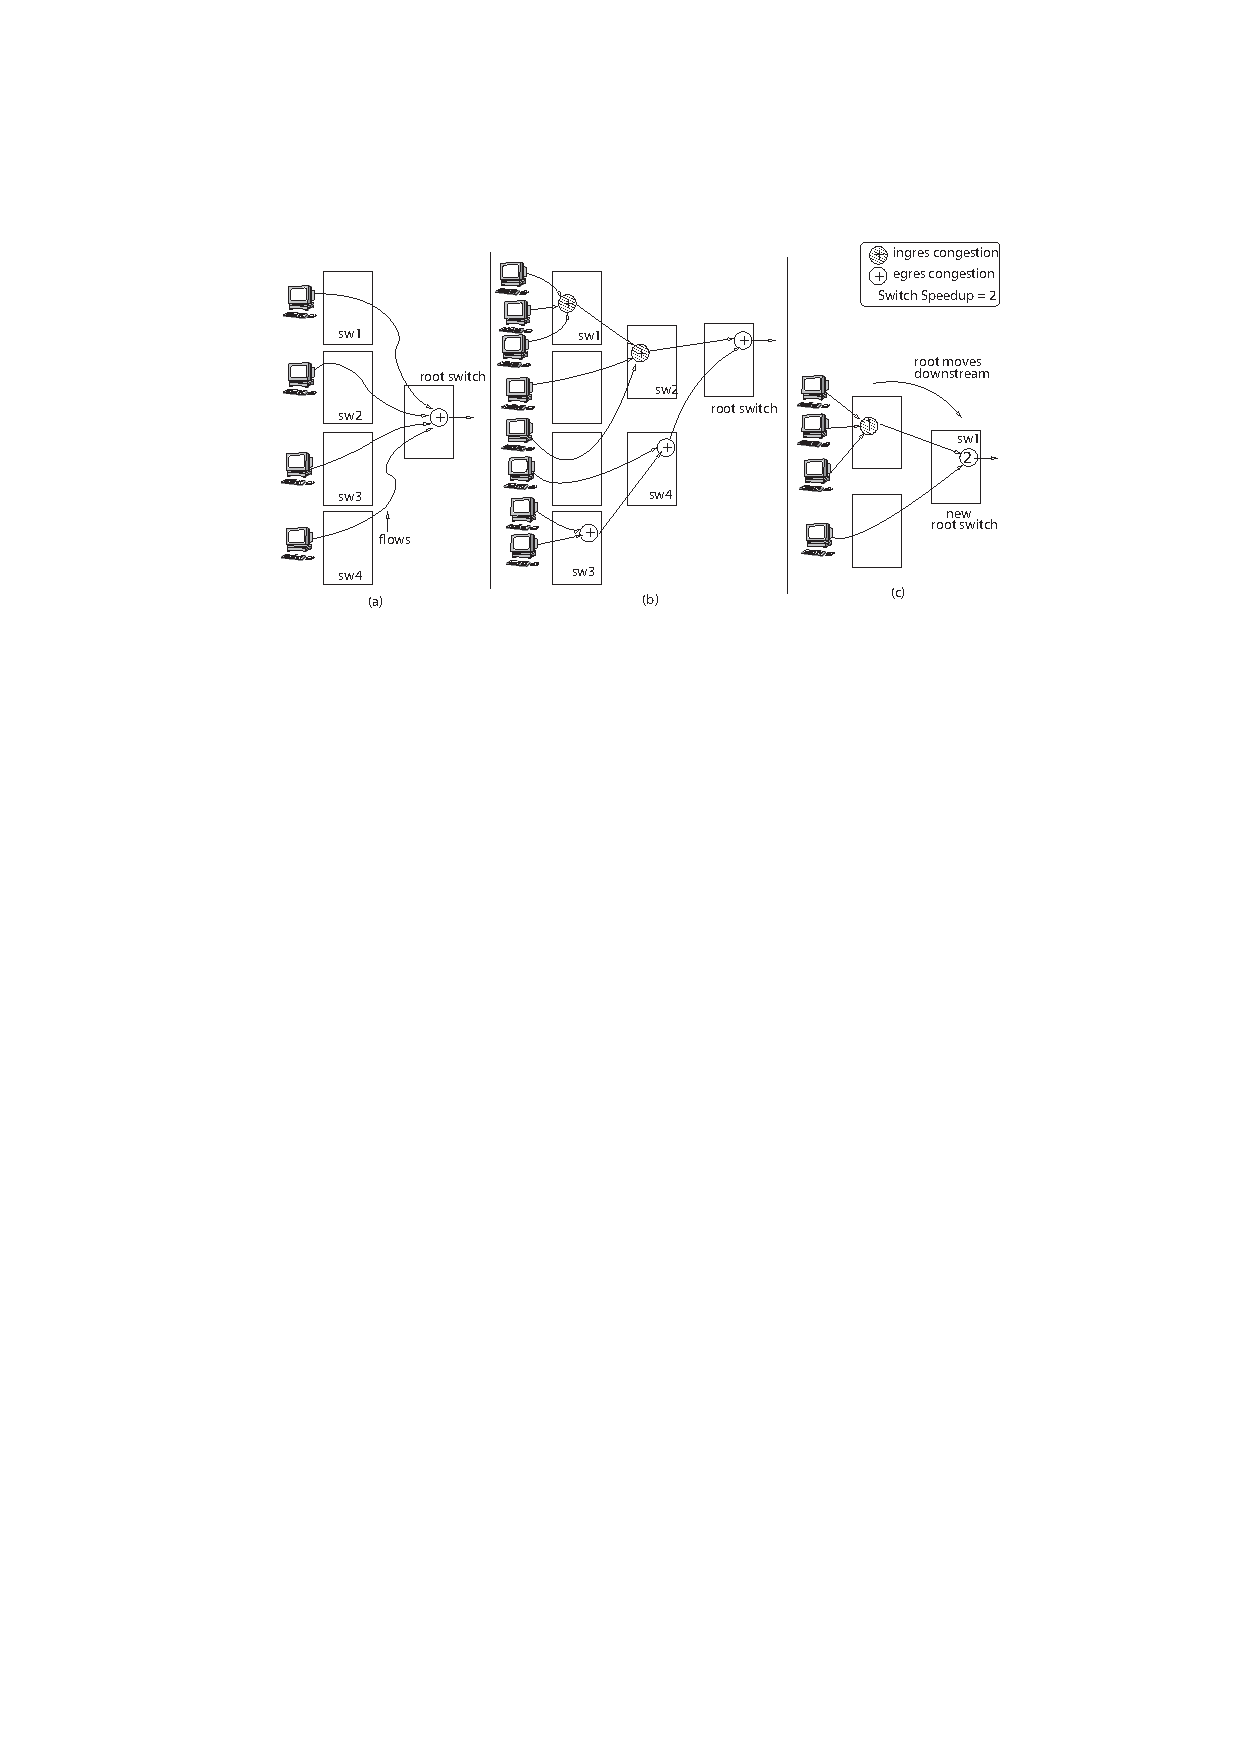
\includegraphics{figures/congestion_dynamics.pdf}
		\caption{Different dynamic formations of trees. Speedup is two. (a) Traditional view about the formation of a congestion tree, (b) Different locations (ingress and egress) where congestion is detected for one tree, and (c) the root switch moves downstream.}
		\label{fig:congestion_dynamics}
\end{figure}

Figure~\ref{fig:congestion_dynamics}.a shows an example of the traditional view: five flows form a congestion tree by meeting at the root switch. The sum of the injection rate of all the flows is higher than the link bandwidth, thus a congestion tree is formed.

\subsection{Effect of Switch Architecture}\label{S:switch_arch}

The formation of a congestion tree is different depending on the number of incoming flows and the rate at which they arrive at a switch. Switch architecture, especially the speedup\footnote{A description of switch speedup is given on page~\pageref{desc:switch_speedup}} of a switch, is also a determining factor as will be shown in the following example. Figure~\ref{fig:speedup_effect} depicts three different situations. In the first one (a), the switch has no speedup and the two flows, injecting at the full rate, are headed to the same destination port. Because a switch without speedup can only handle one packet per cycle, packets are queued at the ingress side. Thus, congestion will occur at the ingress side of the switch. However, if speedup is used (Figure~\ref{fig:speedup_effect}.b) congestion occurs at the egress side. When the number of flows arriving at the root switch is less than or equal to the speedup, the switch can forward the flows to the egress side at the same rate as they are arriving. But, because the output port link speed is only as high as one input link, packets start to queue at the egress side. 

\begin{figure}[ht]
	\centering
		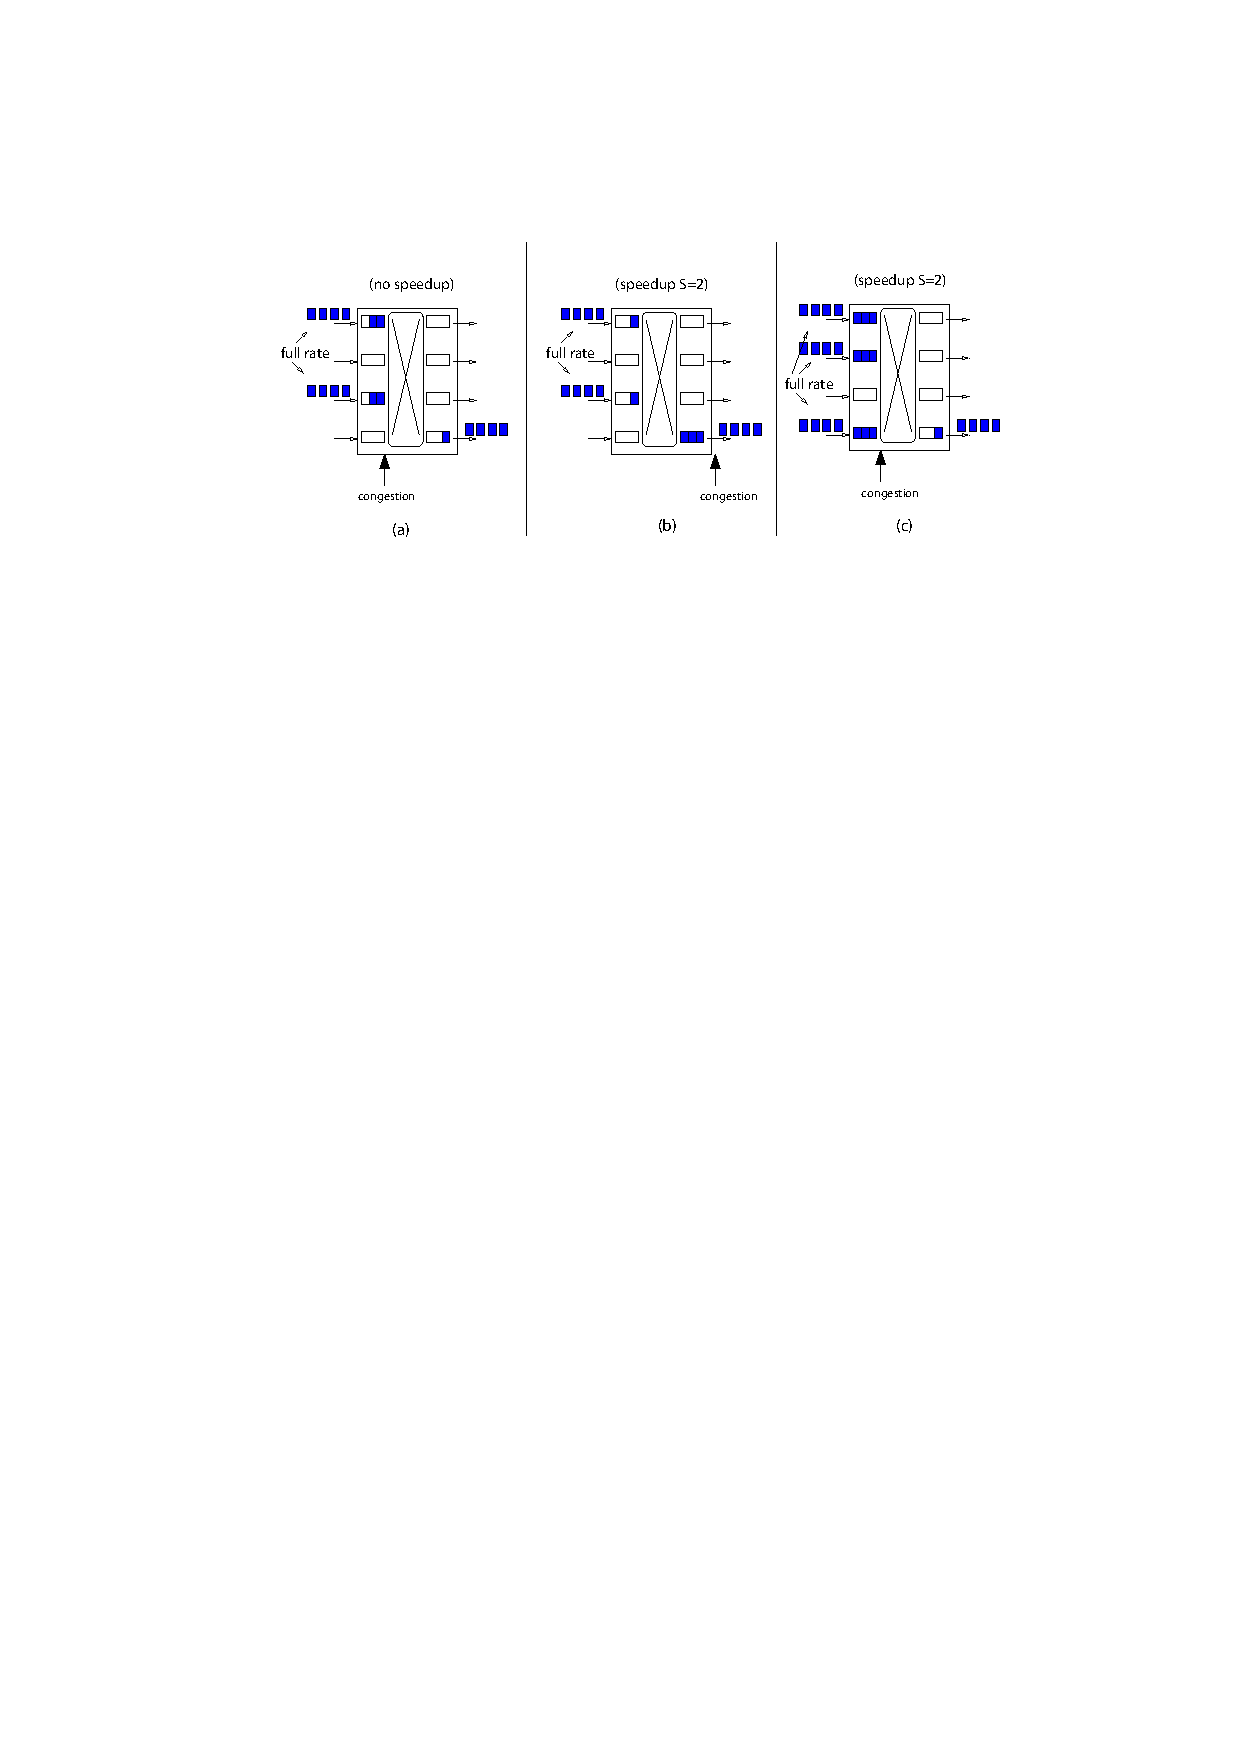
\includegraphics{figures/speedup_effect.pdf}
		\caption{HOL blocking within a switch with different speedups and different flows.}
		\label{fig:speedup_effect}
\end{figure}

Obviously the situation depends on the number of incoming flows and the speedup of the switch. Figure~\ref{fig:speedup_effect}.c illustrates a number of incoming flows higher than the switch speedup, causing the congestion to once again form at the ingress side. Note that congestion will occur regardless of the destination of the incoming flows. 

This effect may also occur at several points along a congestion tree. In figure~\ref{fig:congestion_dynamics}.b we can observe a congestion tree formed by eight flows heading to the same destination. Three flows merge at \emph{sw1}, while other flows merge at different points, finally converging at the root switch. In this situation, congestion first occurs at the ingress side at \emph{sw1} and \emph{sw2}. Once all the flows arrive at the root switch they merge and congestion occurs again. However, in this case, congestion occurs at the egress side, at \emph{sw3}, \emph{sw4} and the root switch.

\subsection{Impact of Traffic Patterns}\label{S:traffic_patterns}

In the previous scenario it was assumed that all the flows were injecting packets at the same rate and started at the same time. This can happen in some cases, such as a barrier synchronization among different processes in a multiprocessor system, but often is not so. Scenarios may arise where different flows contributing to the same congestion tree start at different times and inject at different rates. The authors in~\cite{paper1} describe the more sophisticated dynamics of these scenarios.

They show that the root of a congestion tree may move upstream by the collapse of some branches, or downstream by the addition of new flows. The latter is illustrated in figure~\ref{fig:congestion_dynamics}.b. Also, congestion trees may overlap at several network points without merging. And finally, a congestion tree may be formed from local and transient congestion trees that will later merge due to the limited speedup. Therefore, for all of these cases some kind of architectural support is needed in order to separate each congestion tree and to follow the complex dynamics they may exhibit. 

Now that the dynamics of congestion trees have been explored a bit deeper, we can describe techniques proposed to solve their negative effects.

\section{Proposed Solutions}\label{S:solutions}

In this section we describe three proposed solutions that effectively eliminate HOL blocking and with it, the negative impact of congestion trees on network throughput. First we present a summary of the basic RECN technique by J. Duato et al.~\cite{paper2}. This technique was enhanced by P.J. Garc\'ia et al. in~\cite{paper1}. We state the two enhancements they developed and their achieved performance improvements. Finally this paper includes a brief overview of FBCIM, an adaptation of the RECN approach for networks with table-based, distributed routing~\cite{paper3}. 

\subsection{Basic RECN}\label{S:basic_recn}

RECN stands for regional explicit congestion notification because it detects and explicitly notifies switches about congestion throughout the region that will be affected by a given congestion tree~\cite{paper2}. RECN differs from local explicit congestion notification (LECN) strategies~\cite{KM04} proposed in that it is able to eliminate HOL blocking across multiple stages. The authors in~\cite{paper2} focus on removing HOL blocking in Multistage Interconnection Networks with deterministic routing, effectively making congestion trees harmless. 

The technique basically works by separating the packets from congested flows from the packets belonging to uncongested flows. By doing so, congested packets no longer interfere with uncongested packets and even with packets from congested flows belonging to another tree. This is important since different congested flows usually experience significantly different degrees of congestion. Therefore, the technique focuses on quickly detecting congested flows and immediately mapping them to separate queues. The deallocation of those queues when they are no longer required is also important in order to minimize the number of resources needed to eliminate HOL blocking.

\subsubsection{Congestion Detection}

The congestion detection mechanism is simple, fast and accurately identifies the sources that are contributing to congestion. RECN's congestion detection mechanism consists of detecting when the occupancy of a given output queue reaches a certain threshold. This technique works for both congestion at the endnodes of the network as well as internal network congestion. Fully determining the sources that are contributing to congestion was deemed infeasible due to data RAM bandwidth consumption and the corresponding interference with packet transmission. As such, the authors opted for another approach. The switch simply propagates notifications to the input ports that are contributing to congestion. Each output port has a flag associated with each input port, which records the transmission of the corresponding notification to avoid repeated congestion notifications.

\subsubsection{Congestion Notification and Queue Allocation}

When congestion notifications are received at some input port, a \emph{set aside queue (SAQ)} is locally allocated for the packets leading to the congested output port. All the incoming packets that request the congested output port will be stored in that SAQ, thus preventing them from blocking other packets stored in the main queue for that input port.

Path information is stored in a \emph{content addressable memory (CAM)}. Each CAM line contains the path information associated with the corresponding SAQ. The reason for using a CAM is that the switch has to check the destination address field in the header of every incoming data packet and compare it against all the path informations stored in the CAM to determine whether this packet is going to cross the root of some congestion tree. In such a case, it will be stored in the corresponding SAQ. It should be noted that packets from uncongested flows that will use the same output port at the current switch as other packets from congested flows will not match any CAM line, and therefore, will not be stored in any SAQ, thus avoiding HOL blocking. It is possible that two congestion trees overlap. Moreover, one of them could be a subtree of the other tree. All of these cases are automatically solved when using a CAM to store path information and incoming notification packets are matched against it.

Figure~\ref{fig:cam} shows the CAM structure required to store path information in a switch for PCI Express Advanced Switching\footnote{AS is an open standard for fabric-interconnection technologies developed by the ASI Special Interest Group~\cite{AS}.}. RECN benefits from the routing mechanisms found in AS. In particular, AS uses source deterministic routing. The AS header includes a turn pool made up of 31 bits that contains all the turns (offset from the incoming port to the outgoing port) for every switch along the path. An advantage of this routing method is that it allows to address a particular network point from any other point in the network. Thus, a switch, by inspecting the appropriate turnpool bits of a packet, can know in advance if it will pass through a particular network point.

\begin{figure}[ht]
	\centering
		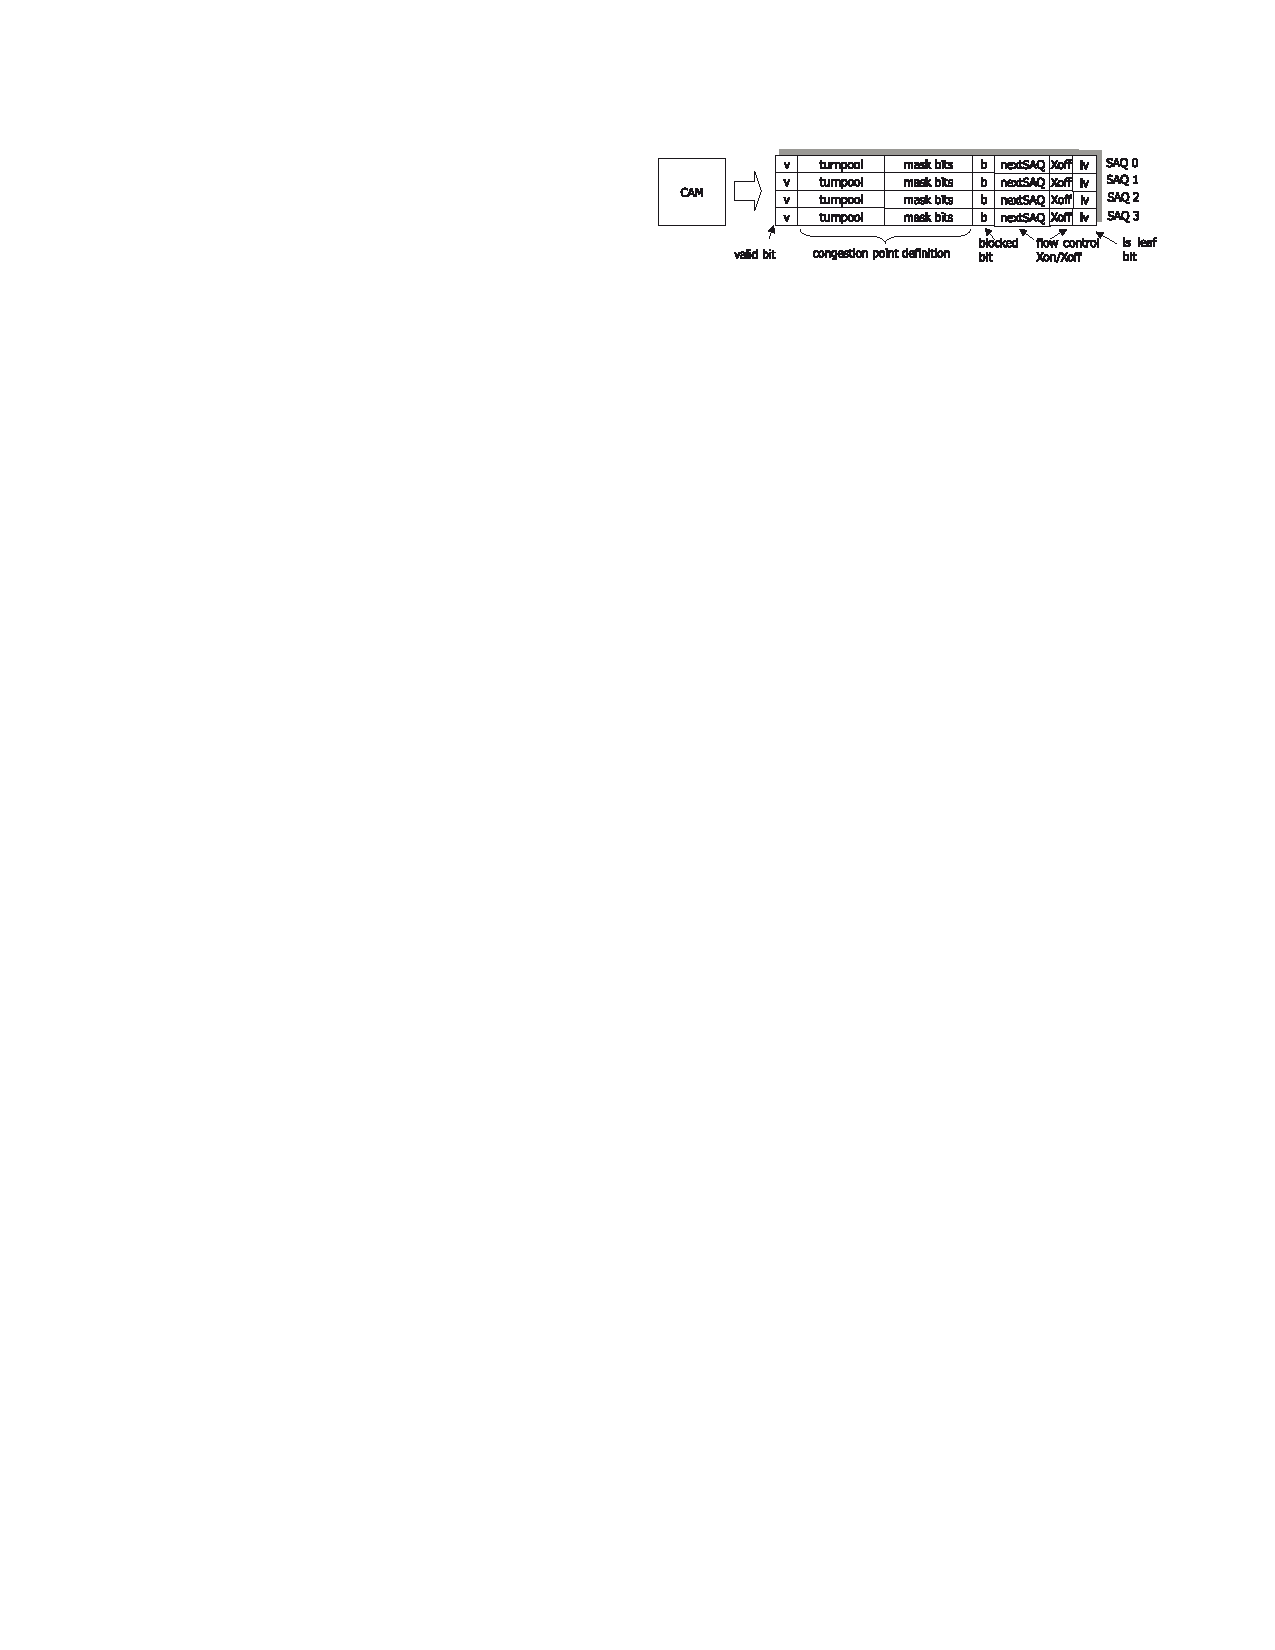
\includegraphics[scale=1.2]{figures/cam.pdf}
		\caption{CAM structure.}
		\label{fig:cam}
\end{figure}

RECN detects congestion \textbf{only} at switch egress ports. When a normal egress queue receives a packet and fills over a given threshold, a notification is sent to the sender ingress port indicating that the output port is congested. This notification includes the routing information (a turnpool and the corresponding mask bits) to reach the congested output port from the notified ingress port. Upon reception of a notification, each ingress port allocates a new SAQ and fills the corresponding CAM line with the received turnpool and mask bits. From that moment, every incoming packet that will pass through the congested point (easily detected from the packet turnpool) will be mapped to the newly allocated SAQ, thus eliminating the HOL blocking it may cause. If an ingress SAQ becomes subsequently congested, a new notification will be sent upstream to some egress port that will react in the same way, allocating an egress SAQ, and so on. As the notifications go upstream, the information indicating the route to the congested point is updated accordingly, in such a way that growing sequences of turns and mask bits are stored in the CAM lines. 

To guarantee in order delivery, whenever a new SAQ is allocated, forwarding packets from that queue is disabled until the last packet of the normal queue (at the moment of the SAQ allocation) is forwarded. This is implemented by a simple pointer associated to the last packet in the normal queue and pointing to the blocked SAQ. RECN also implements for each individual SAQ a special Xon/Xoff flow control, that follows the stop-and-go model. 

RECN keeps track (with a control bit on each CAM line) of the network points that are leaves of a congestion tree. Whenever a SAQ with the leaf bit set to one empties, the queue is deallocated and a notification is sent downstream, repeating the process until the root of the congestion tree is reached. 

\subsection{Enhanced RECN}\label{S:enhancedrecn}

In~\cite{paper2} the authors propose two enhancements to RECN. Both enhancements allow RECN to keep track of the dynamics of congestion trees explored in section~\ref{S:evolution}, and thereby, significantly increase performance.

The first enhancement is allowing RECN to detect congestion at switch ingress ports. Basic RECN defines SAQs at ingress and egress ports, but it only detects congestion at egress ports. However, Section~\ref{S:switch_arch} on page~\pageref{S:switch_arch} shows that congestion may first occur at ingress ports. In these cases, basic RECN never detects congestion at the root. Instead, it detects congestion at the immediate upstream switches, but only when the root ingress queues are full. So, RECN will not react quickly to eliminate HOL blocking at an important part of the tree. 

\begin{figure}[ht]
	\centering
		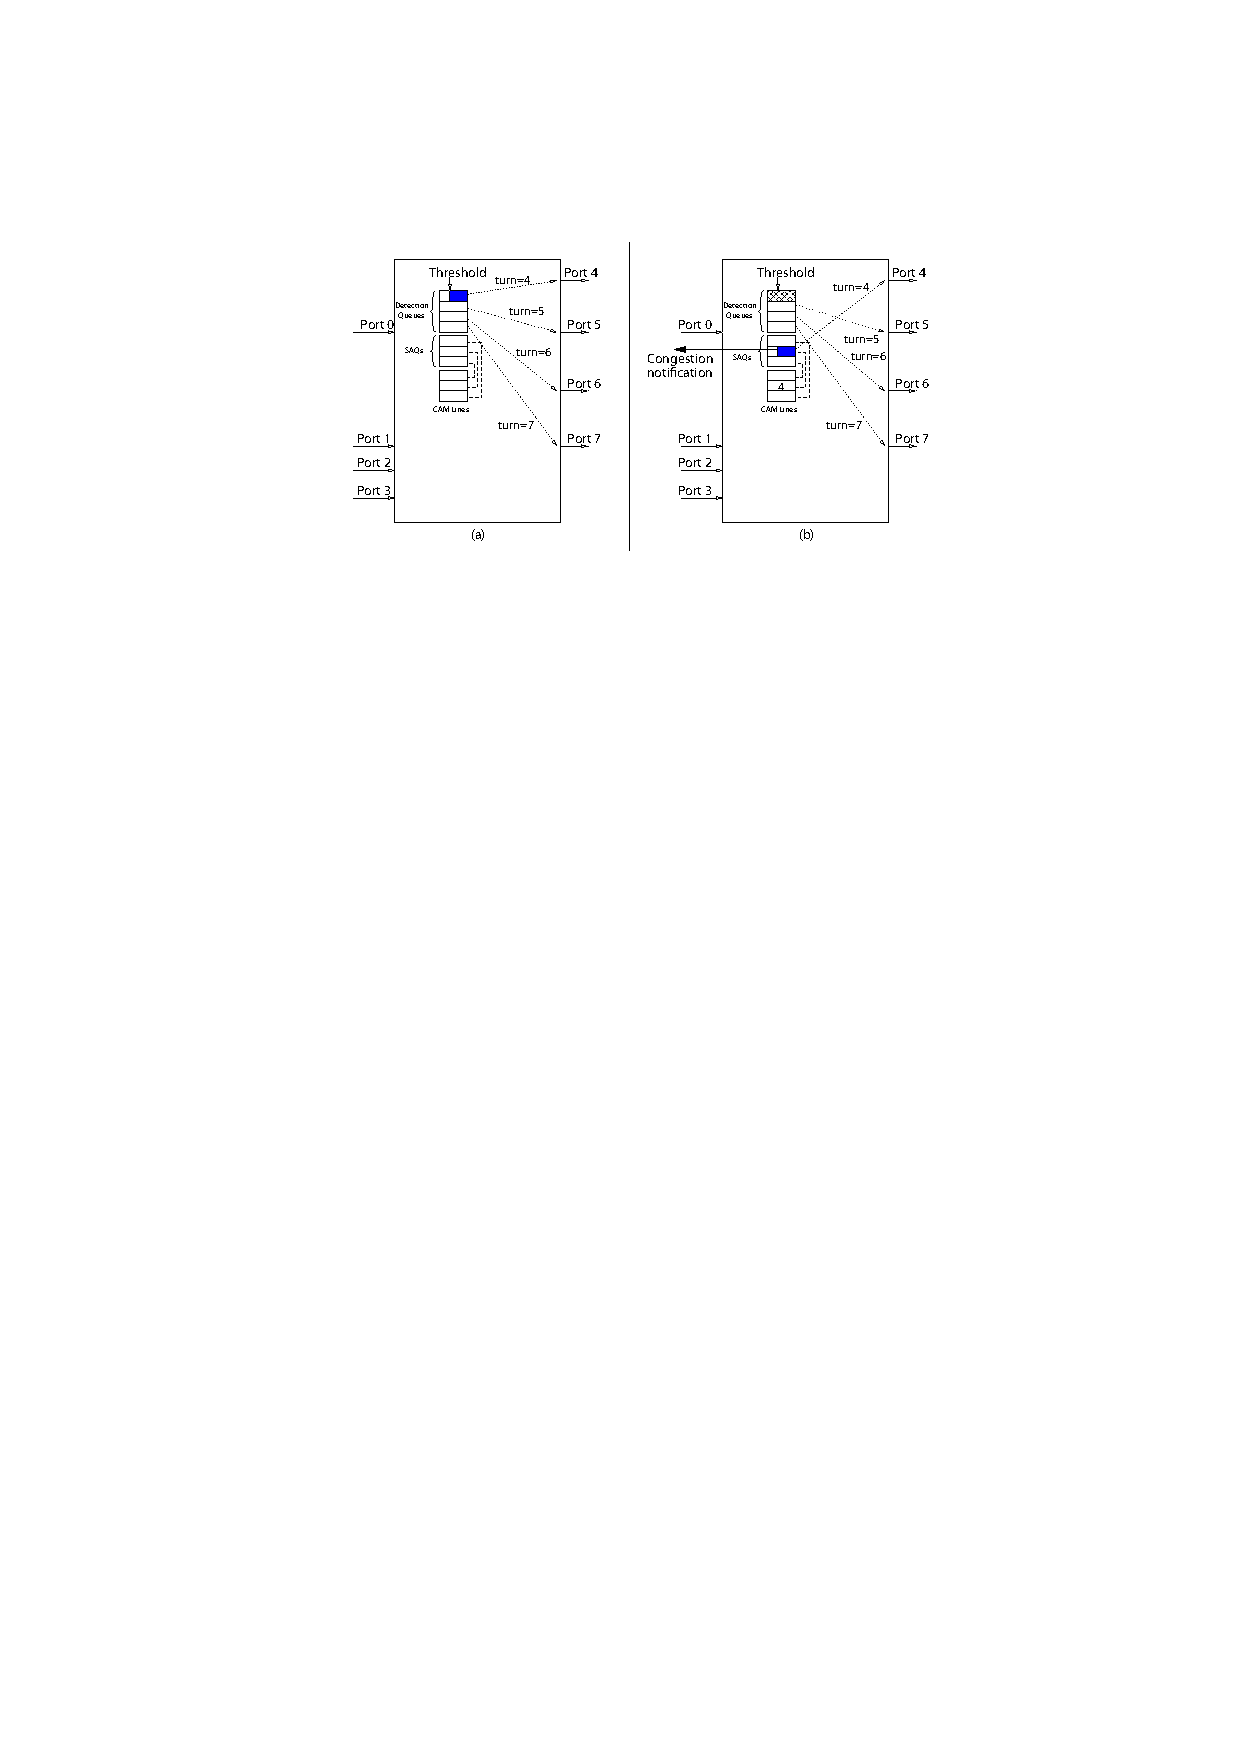
\includegraphics[scale=1.2]{figures/recn1.pdf}
		\caption{Mechanism for detecting and handling congestion at the ingress side: (a) Queue status at the detection moment (b) Queue status after detection.}
		\label{fig:recn1}
\end{figure}

The first enhancement is accomplished by replacing the normal queue at each ingress port by a set of small buffers (referred to as detection queues). So, at ingress ports the memory is now shared by detection queues and SAQs. The detection queues are structured at the switch level: there are as many detection queues as output ports in the switch, and packets heading to a particular output port are directed to the associated detection queue. By doing this, when a detection queue fills over a given threshold, congestion is detected, and the output port causing the congestion is easily computed as the port associated with that detection queue. Once congestion is detected at an ingress port, a new SAQ is allocated at this port, and the turnpool identifying the output port causing congestion is stored in the CAM line. The detection queue where congestion is detected and the SAQ allocated are swapped. As the new SAQ can now be considered to be congested, a notification is sent upstream. Figure~\ref{fig:recn1} shows the proposed mechanism.

\begin{figure}[ht]
	\centering
		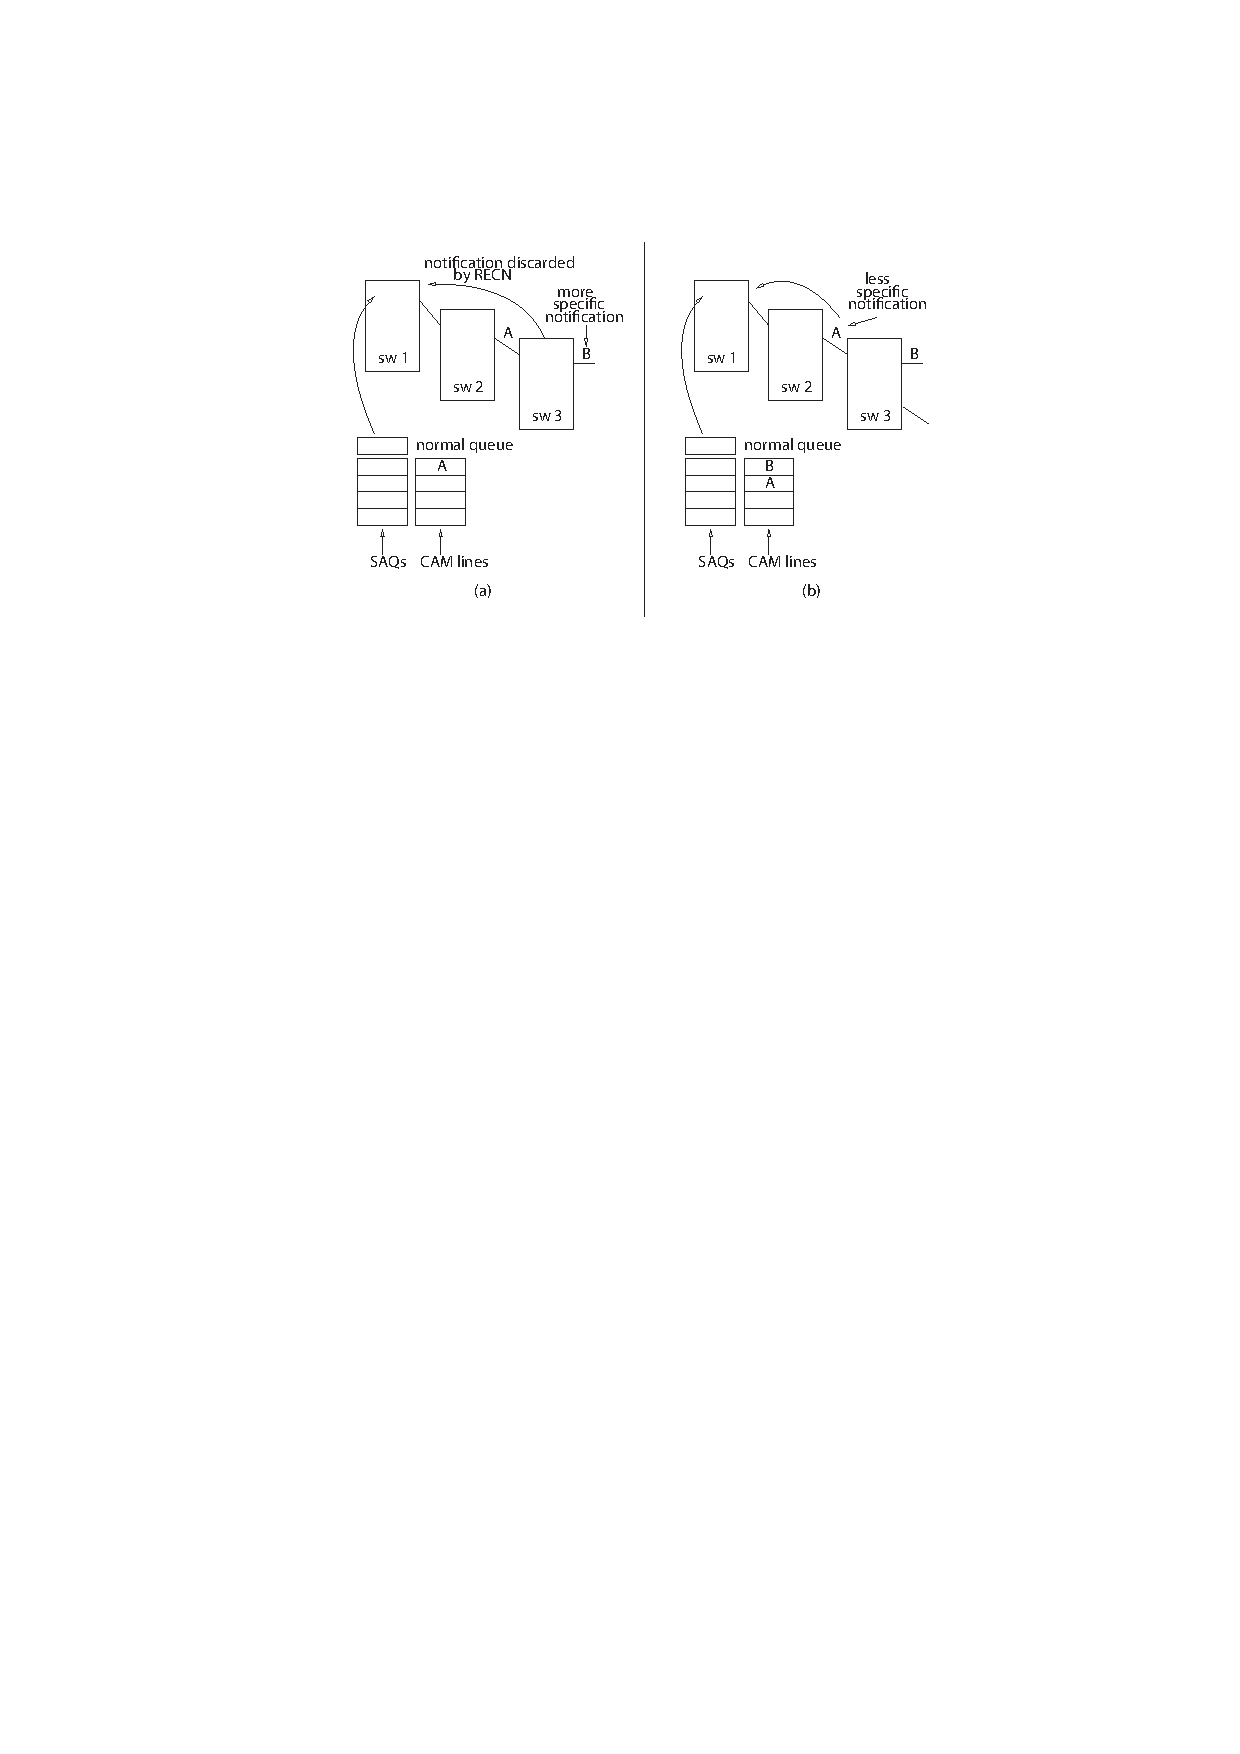
\includegraphics{figures/recn2.pdf}
		\caption{Basic RECN treatment for (a) more specific and (b) less specific notifications.}
		\label{fig:recn2}
\end{figure}

The second enhancement is related to the actions taken upon reception of notifications. Basic RECN does not allocate SAQs for all the notifications received. This is done in order to ensure that no out of order packet delivery is introduced. Figure~\ref{fig:recn2}.a shows an example where RECN does not allocate a SAQ when receiving a notification. First, \emph{sw1} is notified that point A is congested. Then, it allocates a new SAQ for that congested point. Packets going through A will be stored from that moment in that SAQ. Later, point B becomes congested at \emph{sw3} and notifications are sent upstream, reaching \emph{sw1}. This notification is referred to as being a more specific notification (as B is further away than A).

This fact can lead RECN to introduce HOL blocking. Indeed, flows not belonging to the first tree (traffic adressed to point B) passing trough point A will be mapped to the same SAQ (the one associated to A) than flows belonging to the congestion tree. Thus, RECN does not support the downstream tree movement. Also the situation where a congestion tree forms from leaves to root will not be correctly treated.

The second enhancement proposal is to accept all the notifications regardless whether they are more or less specific. In order to deal with out of order issues, when a new SAQ is allocated due to a more specific notification, it must be blocked (must not send packets) until all the packets stored in the SAQ associated to the less specific notification (when the new SAQ is allocated) leave the queue. This can be accomplished by placing a pointer to the new allocated SAQ in the “old” SAQ.

Both enhancements introduced to RECN allow it to detect congestion at ingress ports and allow the system to correctly accommodate for movements of the root switch that are traditionally not taken into consideration. Performance evaluations that highlight the gains provided by these enhancements are reported in section~\ref{S:recn_perf} on page~\pageref{S:recn_perf}.

\subsection{FBICM: Flow-Based Implicit Congestion Management}\label{S:fbicm}

An essential requirement for any RECN implementation is the use of source-based routing where the entire path of a packet is encoded in its header. RECN identifies congested packets by comparing the explicit route stored in the header of each packet to explicit routes leading to congested points. This limitation prevents RECN from being applied in any network technology that uses table-based, distributed routing, like Infiniband~\cite{infiniband}, a high-performance interconnection technology becoming increasingly popular in cluster-based systems.

Flow-Based Implicit Congestion Management (FBICM) was developed in order to bridge this significant technical gap. As RECN, it is able to eliminate HOL blocking produced by congested flows, but it can be employed in networks implementing table-based, distributed deterministic routing. FBICM uses the same basic principles as RECN: detect congested packets and separate them from non-congested ones. The main differences between FBCIM and RECN are:

\newcounter{qcounter}
\begin{list}{\arabic{qcounter}.~}{\usecounter{qcounter}}
\item Congested points are not addressed by means of explicit routes. Instead, FBICM identifies congested points implicitly, by keeping track of the different flows passing through these points.
\item Congested packets are not identified as packets following an explicit route to a congested point, but as packets belonging to flows involved in a congested situation.
\item Congestion information is associated to destinations where as in RECN it is associated
to internal network points.
\end{list}

For a detailed description of FBCIM, including switch architecture and operation examples, please refer to~\cite{paper3}. The paper further describes how implicit information about congested points can be stored and propagated (once congestion is detected) without requiring explicit routes, and how packets belonging to congested flows can be identified taking into account just their destination.

\section{Performance Evaluation}\label{S:performance}

The original performance analysis of basic RECN was revealed in~\cite{paper2}, the improvements introduced by the enhanced RECN in~\cite{paper1} and the original authors of FBCIM uncovered their benchmark results in~\cite{paper3}. All three used a custom developed detailed event-driven simulator that allowed them to model the network at the register transfer level. For a thorough description of the simulator we recommend section 5.1 of~\cite{paper1}.

As all three papers elaborate their performance evaluation to a great detail, we only present the general facts and highlight some interesting outcomes.

\subsection{RECN Performance}\label{S:recn_perf}

RECN was tested with two different scenarios: using well-defined synthetic traffic patterns and using I/O traces provided by Hewlett-Packard Labs\footnote{HP Storage Systems Program, \url{http://www.hpl.hp.com/research/ssp/software/}.}. 

Figure~\ref{fig:recn_perf_1} shows interesting results for basic RECN, enhanced RECN and VOQsw (Virtual Output Queuing at switch level). A crossbar speedup of 1.5 is used. Time is plotted on the horizontal axis, while network throughput is displayed on the vertical axis. It can be noticed that the basic RECN mechanism starts to degrade performance as throughput drops from 44 bytes/ns to 37 bytes/ns. However, when the congestion tree disappears, performance recovers, although exhibiting a significant oscillation, due to the fact that HOL blocking is not completely eliminated. On the other hand, enhanced RECN behaves optimally as it tolerates the congestion tree with no performance degradation. 

\begin{figure}[ht]
	\centering
		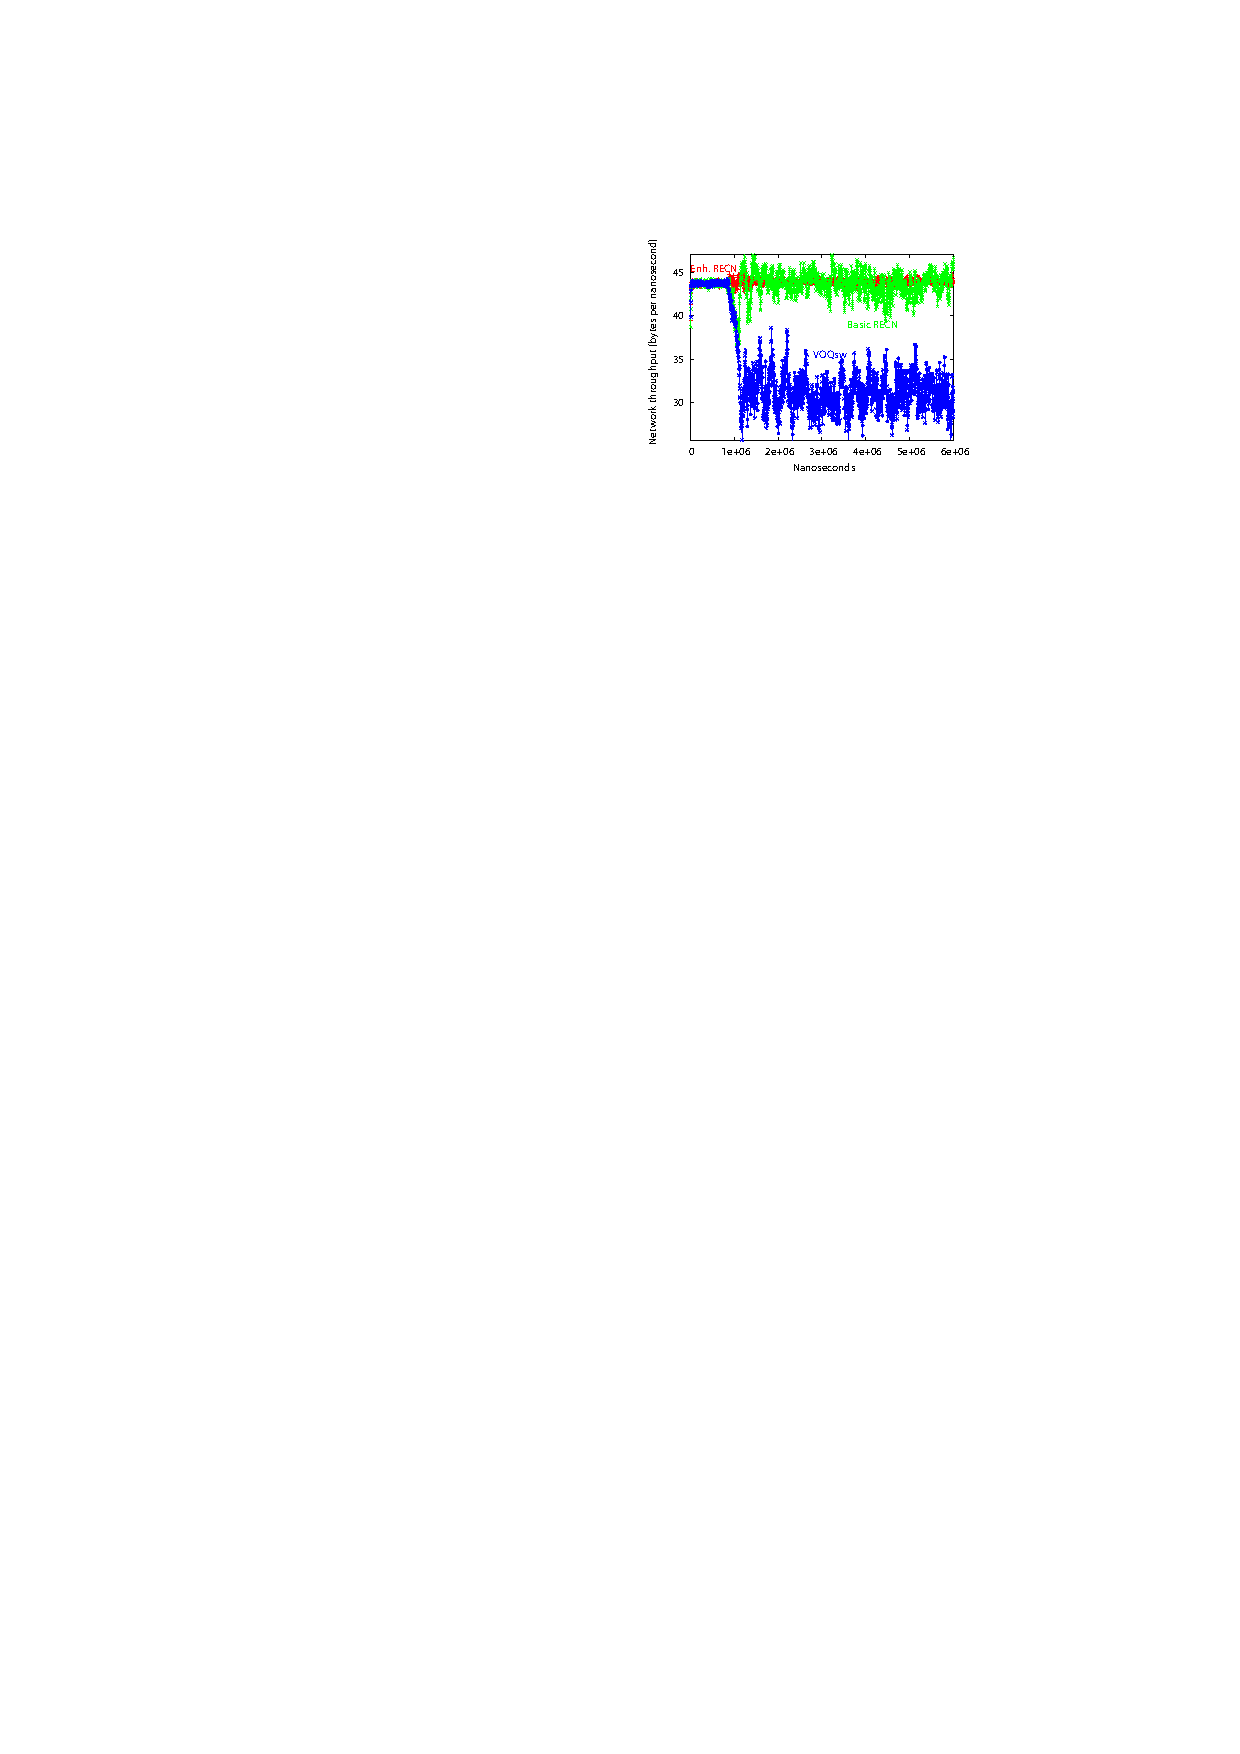
\includegraphics[scale=1.5]{figures/recn_perf_1.pdf}
		\caption{Network throughput with 1.5 speedup for RECN and VOQsw}
		\label{fig:recn_perf_1}
\end{figure}

Taking the throughput results of VOQsw as a reference, it can be deduced that both RECN versions handle the congestion caused by this specific traffic case very well, whereas the performance achieved by VOQsw is quite poor. Looking at both the performance of basic and enhanced RECN, we can conclude that the use of any of them virtually eliminates HOL blocking and that they perform a lot better than the reference VOQsw.

Figure~\ref{fig:recn_perf_2} highlights a situation where the enhancements proposed to RECN are clearly beneficial. It depicts the throughput of the SAN\footnote{Storage Area Network} traces provided by HP, using no speedup when a sudden congestion tree forms. As can be observed, the basic RECN suffers from severe degradation: network throughput drops from  44 bytes/ns to 10 bytes/ns (a 77\% drop). Also noticeable is the fact that basic RECN recovery time is quite excessive and that it never fully recovers. Enhanced RECN on the other hand is able to withstand the absence of speedup and the dynamics of congestion trees, achieving maximum performance. It seems to handle this workload without a hitch by completely eliminates HOL blocking, even at the ingress ports.

\begin{figure}[ht]
	\centering
		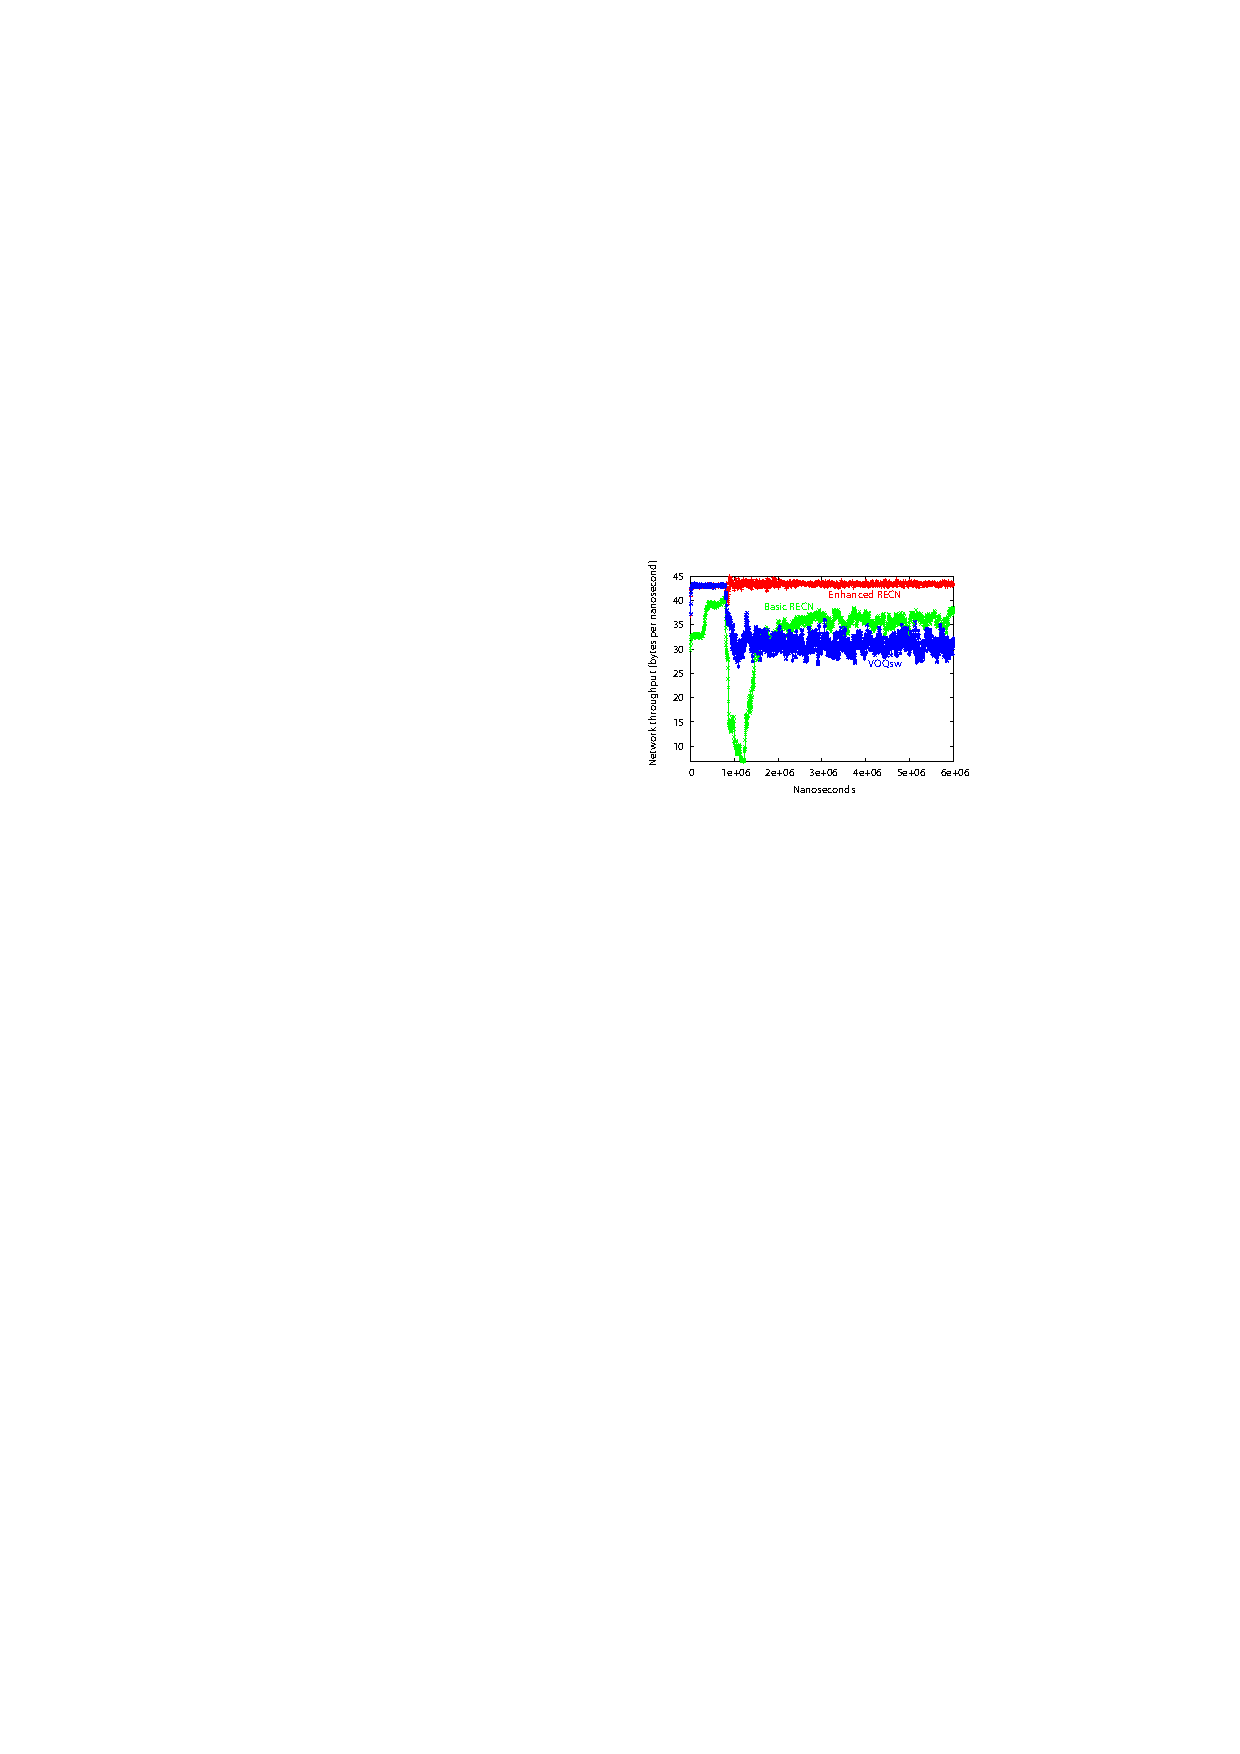
\includegraphics[scale=1.5]{figures/recn_perf_2.pdf}
		\caption{Network throughput without speedup for SAN traces.}
		\label{fig:recn_perf_2}
\end{figure}

Further test in~\cite{paper2} reveal that for large networks (${2048 \times 2048}$ MINs) the effects of the enhanced RECN are even more pronounced. Again, the interested reader caring for the full picture should consult the entire results.

\subsection{FBCIM Performance}\label{S:fbcim_perf}

The evaluation of FBCIM in~\cite{paper3} states that maximum performance is achieved by FBICM regardless of network size or traffic pattern, even in congestion situations. Virtual Output Queues at network level (VOQNet) obtains similar results than FBICM, but requires far more resources, especially in large networks. VOQSw consumes similar resources than FBICM, but its performance is poor in hot-spot traffic situations, regardless of network size. As can be expected, results for FBICM are similar to the RECN ones, but in a different interconnect context. We refer to~\cite{paper3} for the full evaluation.

\section{Conclusion}\label{S:conclusion}

This paper started by explored the complex nature of the formation of congestion trees in networks with CIOQ switches. It presented examples showing that, contrary to the common belief, a congestion tree can grow in a variety of ways, depending on switch architecture (crossbar speedup) and traffic load. 

We also showed that congestion situations are a serious threat to the performance of interconnection networks. In these situations, packet flows contributing to congestion slow the advance of other flows due to HOL blocking, effectively degrading overall network performance. Many techniques have been proposed to solve this problem. Basic RECN accomplishes decent results, and with the enhancements described in section~\ref{S:enhancedrecn} it achieves great performance by eliminating HOL blocking in a truly efficient and scalable way. 

Since RECN requires the use of deterministic source routing, networks using table-based, distributed deterministic routing cannot benefit from a RECN implementation. For these types of networks FBCIM offers an equally performing solution. The performance of FBCIM is on par with the RECN and far better than other solutions. 

\begin{thebibliography}{99}

\bibitem{paper2} J. Duato, I. Johnson, J. Flich, F. Naven, P. Garc\'ia, and T. Nachiondo \emph{A New Scalable and Cost-Effective Congestion Management Strategy for Lossless Multistage Interconnection Networks}, 2005.

\bibitem{paper1} P.J. Garc\'ia, J. Flich, J. Duato, I. Johnson, F.J. Quiles, F. Naven, \emph{Dynamic Evolution of Congestion Trees: Analysus and Impact on Switch Architecture}, 2005.

\bibitem{paper3} J. Escudero-Sahuquillo, P.J. Garc\'ia, F.J.  Quiles, J. Flich, and J. Duato, \emph{FBICM: Efficient Congestion Management for High-Performance Networks Using Distributed Deterministic Routing}, 2008.

\bibitem{myrinet} Myrinet 2000 Series	 Networking.\\
Available at 
\url{http://www.myricom.com/myrinet/overview/}.

\bibitem{infiniband} InfiniBand Trade Association, \emph{InfiniBand Architecture. Specification Volume 1. Release 1.0}. Available at \url{http://www.infinibandta.org}.

\bibitem{SPJ03} L. Shang, L. S. Peh, and N. K. Jha, \emph{Dynamic Voltage Scaling with Links for Power Optimization of Interconnection Networks}, in Proc. Int. Symp. on High-Performance Computer
Architecture, pp. 91--102, Feb. 2003.

\bibitem{hol_thoughput} M. Karol, M. Hluchyj, S. Morgan, \emph{Input Versus Output Queuing on a Space-Division Packet Switch}, IEEE Transactions on Communications, Volume 35, Issue 12, pp. 1347--1356, Dec 1987.

\bibitem{PN85} G. Pfister and A. Norton, \emph{Hot Spot Contention and Combining in Multistage Interconnect Networks}, IEEE Trans. on Computers, vol. C-34, pp. 943--948, Oct. 1985.

\bibitem{pD99} S. P. Dandamudi, \emph{Reducing Hot-Spot Contention in Shared-Memory Multiprocessor Systems},in IEEE Concurrency, vol. 7, no 1, pp. 48--59, January 1999.

\bibitem{BLKC93} R. Bianchini, T. J. LeBlanc, L. I. Kontothanassis, M. E. Crovella, \emph{Alleviating Memory Contention in Matrix Computations on Large-Scale Shared-Memory Multiprocessors}, Technical report 449, Dept. of Computer Science, Rochester University, April 1993.

\bibitem{YTL87} P. Yew, N. Tzeng, D.H. Lawrie, \emph{Distributing Hot-Spot Addressing in Large-Scale Multiprocessors},IEEE Transactions on Computers, vol. 36, no. 4, pp. 388--395, April 1987.

\bibitem{WSNA95} M. Wang, H. J. Siegel, M. A. Nichols, S. Abraham, \emph{Using a Multipath Network for Reducing the Effects of Hot Spots}, IEEE Transactions on Parallel and Distributed Systems, vol. 6, no.3, pp. 252--268, March 1995.

\bibitem{HE89} W.S. Ho, D.L. Eager, \emph{A Novel Strategy for Controlling Hot Spot Contention}, in Proc. Int. Conf. Parallel Processing, vol. I, pp. 14--18, 1989.

\bibitem{AG94} G.S. Almasi, A. Gottlieb, \emph{Highly parallel computing}, 1994.

\bibitem{SS90} S.L. Scott, G.S. Sohi, \emph{The Use of Feedback in Multiprocessors and Its Application to Tree Saturation Control}, IEEE Transactions on Parallel Distributed Systems, vol. 1, no. 4, pp.385--398, Oct. 1990.

\bibitem{TLM01} M. Thottethodi, A. R. Lebeck, S. S. Mukherjee, \emph{Self-Tuned Congestion Control for Multiprocessor Networks}, in Proc. Int. Symp. High-Performance Computer Architecture, Feb. 2001.

\bibitem{V00} W. Vogels et al, \emph{Tree-Saturation Control in the AC3 Velocity Cluster Interconnect}, in Proc. 8th Conference on Hot Interconnects, Aug. 2000.

\bibitem{KLC97} J. H. Kim, Z. Liu, and A. A. Chien, \emph{Compressionless Routing: A Framework for Adaptive and Fault-Tolerant Routing}, IEEE Trans. on Parallel and Distributed Systems, vol. 8, no. 3, 1997.

\bibitem{LSC95} J. Liu, K.G. Shin, C.C. Chang, \emph{Prevention of Congestion in Packet-Switched Multistage Interconnection Networks}, IEEE Transactions on Parallel Distributed Systems, vol. 6, no. 5, pp. 535--541, May 1995.

\bibitem{BLD01} E. Baydal,P. L\'opez and J.Duato, \emph{A Congestion Control Mechanism for Wormhole Networks}, in Proc. 9th. Euromicro Workshop Parallel and Distributed Processing, pp. 19--26, Feb. 2001.

\bibitem{LD93} P. L\'opez and J. Duato, \emph{Deadlock-Free Adaptive Routing Algorithms for the 3D-Torus: Limitations and Solutions}, in Proc. Parallel Architectures and Languages Europe 93, June 1993.

\bibitem{KM04} V. Krishnan and D. Mayhew, \emph{A Localized Congestion Control Mechanism for PCI Express Advanced Switching Fabrics}, in Proc. 12th IEEE Symp. on Hot Interconnects, Aug. 2004.

\bibitem{AS} \emph{Advanced Switching for the PCI Express Architecture}. White paper.\\
Available at \url{http://www.intel.com/technology/pciex press/devnet/AdvancedSwitching.pdf}

\end{thebibliography}

\end{document}%% LaTeX - Article customise

